% LuminaFPM figure library. Each figure is delimited by %%BEGINFIG:<label>%% ... %%ENDFIG%%
% and inlined by the assembler at the matching %%FIG:<label>%% marker. Delimiters are
% stripped during assembly (they never reach the final document).

%%BEGINFIG:fig:pipeline%%
\begin{figure}[htbp]
\centering
\begin{tikzpicture}[
  stage/.style={draw=black!70, rounded corners, fill=LightGray, text width=10.6cm, align=center, minimum height=7.4mm, font=\small},
  node distance=4.4mm]
\node[stage] (s1) {1.~Acquisition --- read-only poll: FortiGate REST/JSON, Palo Alto PAN-OS XML};
\node[stage, below=of s1] (s2) {2.~Parsing --- vendor payloads parsed into structured intermediate objects};
\node[stage, below=of s2] (s3) {3.~Normalization --- single canonical multi-vendor policy model};
\node[stage, below=of s3] (s4) {4.~Repository --- PostgreSQL normalized store (source of truth)};
\node[stage, below=of s4] (s5) {5.~Deterministic Anomaly Engine --- set-theoretic detection on normalized rules};
\node[stage, below=of s5] (s6) {6.~Risk Scoring --- composite 0--100 score, factors, tiers};
\node[stage, below=of s6] (s7) {7.~Threat Intelligence --- API-based indicator enrichment (data-minimized)};
\node[stage, below=of s7] (s8) {8.~AI Reporting --- LLM evidence-grounded SOC report (explains, never detects)};
\node[stage, below=of s8] (s9) {9.~Dashboard --- React/TypeScript visualization and analyst workflow};
\foreach \a/\b in {s1/s2,s2/s3,s3/s4,s4/s5,s5/s6,s6/s7,s7/s8,s8/s9}
  \draw[-{Latex[length=2mm]}, thick] (\a) -- (\b);
\end{tikzpicture}
\caption{The LuminaFPM end-to-end processing pipeline (nine logical layers).}
\label{fig:pipeline}
\end{figure}
%%ENDFIG%%

%%BEGINFIG:fig:arch%%
\begin{figure}[htbp]
\centering
\begin{tikzpicture}[
  layer/.style={draw=black!70, rounded corners, fill=LightGray, text width=12.6cm, align=center, minimum height=11mm, font=\small},
  node distance=3.4mm]
\node[layer] (l1) {\textbf{Presentation Layer}\\React + TypeScript + Vite SPA --- dashboard, policy audit, risk, reports, CTI, topology, benchmark};
\node[layer, below=of l1] (l2) {\textbf{API Layer}\\FastAPI REST endpoints (vendors, devices, rules, anomalies, risk, cti, reports, benchmark)};
\node[layer, below=of l2] (l3) {\textbf{Application / Services Layer}\\acquisition $\cdot$ parsing $\cdot$ normalization $\cdot$ anomaly engine $\cdot$ risk $\cdot$ CTI $\cdot$ LLM reporting $\cdot$ benchmark};
\node[layer, below=of l3] (l4) {\textbf{Asynchronous Workers}\\Celery tasks (acquire / normalize / analyze) coordinated through a Redis broker};
\node[layer, below=of l4] (l5) {\textbf{Data and Integration Layer}\\PostgreSQL normalized repository $\cdot$ Fernet-encrypted credentials $\cdot$ LLM and CTI providers};
\foreach \a/\b in {l1/l2,l2/l3,l3/l4,l4/l5}
  \draw[{Latex[length=2mm]}-{Latex[length=2mm]}, thick] (\a) -- (\b);
\end{tikzpicture}
\caption{Layered system architecture of LuminaFPM.}
\label{fig:arch}
\end{figure}
%%ENDFIG%%

%%BEGINFIG:fig:labtopo%%
\begin{figure}[htbp]
\centering
\begin{tikzpicture}[
  dev/.style={draw=black!70, rounded corners, fill=LightGray, align=center, minimum width=2.7cm, minimum height=10mm, font=\footnotesize},
  sub/.style={draw=black!70, rounded corners, fill=white, align=center, minimum width=2.7cm, minimum height=9mm, font=\footnotesize},
  net/.style={draw=black!55, dashed, rounded corners, inner sep=4mm}]
\node[dev] (fgt)  at (0,0)    {FortiGate VM\\192.168.55.10};
\node[dev] (pa)   at (4.2,0)  {Palo Alto VM\\192.168.55.20};
\node[dev] (kali) at (8.4,0)  {Kali (attacker)\\192.168.55.100};
\node[dev] (lum)  at (4.2,-2.5) {LuminaFPM host\\192.168.55.1};
\node[sub] (lan)  at (0,-5.0)  {LAN\\10.10.10.0/24};
\node[sub] (dmz)  at (4.2,-5.0) {DMZ\\10.10.20.0/24};
\node[sub] (db)   at (8.4,-5.0) {DB\\10.10.30.0/24};
\begin{scope}[on background layer]
  \node[net, fit=(fgt)(pa)(kali), label={[font=\footnotesize]above:Management network --- 192.168.55.0/24}] {};
  \node[net, fit=(lan)(dmz)(db), label={[font=\footnotesize]below:Shared data-plane subnets}] {};
\end{scope}
\draw[-{Latex[length=2mm]}, thick] (lum) -- node[left, font=\scriptsize]{poll (RO)} (fgt);
\draw[-{Latex[length=2mm]}, thick] (lum) -- node[right, font=\scriptsize]{poll (RO)} (pa);
\end{tikzpicture}
\caption{Parallel shared-network virtual laboratory topology. LuminaFPM polls both firewalls read-only over the management network; the firewalls independently govern the shared data-plane subnets.}
\label{fig:labtopo}
\end{figure}
%%ENDFIG%%

%%BEGINFIG:fig:context%%
\begin{figure}[htbp]
\centering
\begin{tikzpicture}[
  sys/.style={draw=black!80, very thick, rounded corners, fill=LightGray, align=center, minimum width=3.6cm, minimum height=1.6cm, font=\small},
  ext/.style={draw=black!70, align=center, minimum width=2.7cm, minimum height=10mm, font=\footnotesize},
  flow/.style={-{Latex[length=2mm]}, thick}]
\node[sys] (s)   at (0,0)     {LuminaFPM\\Firewall Anomaly\\Management Platform};
\node[ext] (fgt) at (-5.2,1.7)  {FortiGate};
\node[ext] (pa)  at (-5.2,-1.7) {Palo Alto};
\node[ext] (an)  at (5.2,1.9)   {Security Analyst};
\node[ext] (llm) at (5.2,-0.1)  {LLM Provider\\(Gemini)};
\node[ext] (cti) at (5.2,-2.1)  {CTI Providers};
\draw[flow] (fgt) -- node[above, font=\scriptsize]{config (RO)} (s);
\draw[flow] (pa)  -- node[below, font=\scriptsize]{config (RO)} (s);
\draw[flow] (s)   -- node[above, font=\scriptsize]{findings / reports} (an);
\draw[flow] (s)   -- node[above, font=\scriptsize]{prompt} (llm);
\draw[flow] (s)   -- node[below, font=\scriptsize]{indicators} (cti);
\end{tikzpicture}
\caption{Context diagram: LuminaFPM and its external entities. All firewall interaction is strictly read-only.}
\label{fig:context}
\end{figure}
%%ENDFIG%%

%%BEGINFIG:fig:dfd%%
\begin{figure}[htbp]
\centering
\begin{tikzpicture}[
  proc/.style={draw=black!70, circle, fill=LightGray, align=center, minimum size=1.6cm, font=\scriptsize, inner sep=1pt},
  ent/.style={draw=black!70, align=center, minimum width=2.1cm, minimum height=8mm, font=\footnotesize},
  store/.style={draw=black!70, align=center, minimum width=4.6cm, minimum height=8mm, font=\footnotesize},
  flow/.style={-{Latex[length=2mm]}}]
\node[ent]   (fw) at (-5.2,1)  {Firewalls};
\node[ent]   (an) at (-5.2,-2.2) {Analyst};
\node[proc]  (p1) at (-1.6,0.6) {1. Acquire \&\\Normalize};
\node[proc]  (p2) at (1.8,0.6)  {2. Detect\\Anomalies};
\node[proc]  (p3) at (1.8,-2.2) {3. Score \&\\Enrich (CTI)};
\node[proc]  (p4) at (-1.6,-2.2){4. Report\\(LLM)};
\node[store] (db) at (0.1,-4.1) {D1: PostgreSQL normalized repository};
\draw[flow] (fw) -- node[above,font=\scriptsize]{raw config} (p1);
\draw[flow] (p1) -- node[above,font=\scriptsize]{normalized rules} (p2);
\draw[flow] (p2) -- node[right,font=\scriptsize]{findings} (p3);
\draw[flow] (p3) -- node[above,font=\scriptsize]{risk + exposure} (p4);
\draw[flow] (p4) -- node[above,font=\scriptsize]{report} (an);
\draw[flow] (p1) -- (db);
\draw[flow] (db) -- (p2);
\draw[flow] (p3) -- (db);
\end{tikzpicture}
\caption{Data flow diagram of the LuminaFPM analysis pipeline.}
\label{fig:dfd}
\end{figure}
%%ENDFIG%%

%%BEGINFIG:fig:erd%%
\begin{figure}[htbp]
\centering
\resizebox{\linewidth}{!}{%
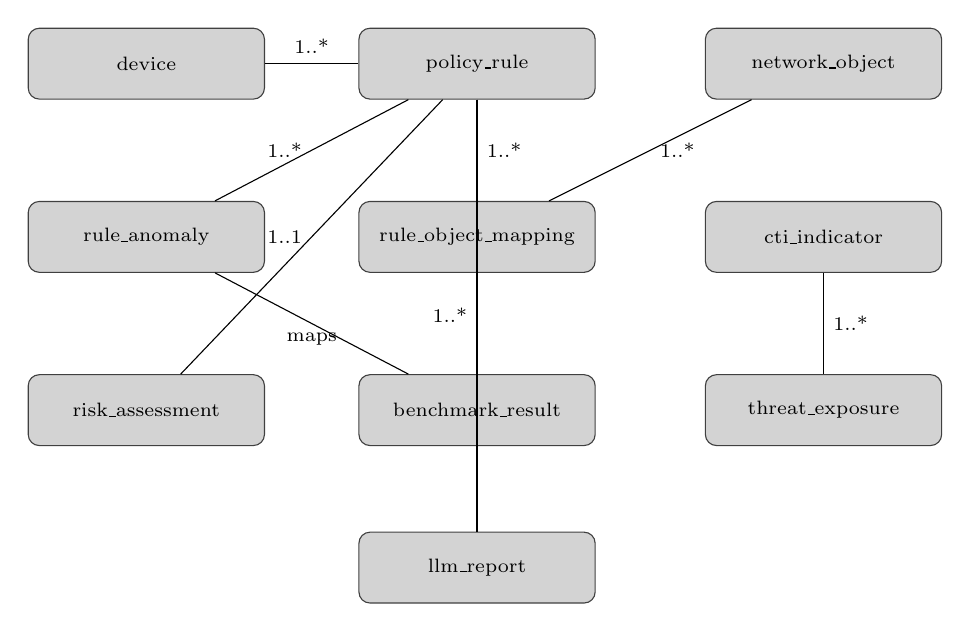
\begin{tikzpicture}[
  ent/.style={draw=black!75, rounded corners, fill=LightGray, align=center, minimum width=3.0cm, minimum height=9mm, font=\scriptsize},
  rel/.style={font=\scriptsize, midway}]
\node[ent] (dev)  at (0,0)    {device};
\node[ent] (rule) at (4.2,0)  {policy\_rule};
\node[ent] (obj)  at (8.6,0)  {network\_object};
\node[ent] (anom) at (0,-2.2) {rule\_anomaly};
\node[ent] (map)  at (4.2,-2.2) {rule\_object\_mapping};
\node[ent] (cti)  at (8.6,-2.2) {cti\_indicator};
\node[ent] (risk) at (0,-4.4) {risk\_assessment};
\node[ent] (bench)at (4.2,-4.4) {benchmark\_result};
\node[ent] (texp) at (8.6,-4.4) {threat\_exposure};
\node[ent] (rep)  at (4.2,-6.4) {llm\_report};
\draw (dev)  -- node[rel,above]{1..*} (rule);
\draw (rule) -- node[rel,right]{1..*} (map);
\draw (obj)  -- node[rel,right]{1..*} (map);
\draw (rule) -- node[rel,left]{1..*} (anom);
\draw (rule) -- node[rel,left]{1..1} (risk);
\draw (cti)  -- node[rel,right]{1..*} (texp);
\draw (anom) -- node[rel,below]{maps} (bench);
\draw (rule) -- node[rel,left]{1..*} (rep);
\end{tikzpicture}}
\caption{Entity--relationship diagram of the normalized policy and analysis schema (core entities).}
\label{fig:erd}
\end{figure}
%%ENDFIG%%

%%BEGINFIG:fig:anomflow%%
\begin{figure}[htbp]
\centering
\begin{tikzpicture}[
  node distance=7mm,
  term/.style={draw=black!75, rounded rectangle, fill=LightGray, font=\footnotesize, align=center, minimum height=7mm, inner sep=4pt},
  box/.style={draw=black!75, fill=LightGray, text width=5.4cm, align=center, font=\footnotesize, minimum height=8mm},
  dec/.style={draw=black!75, diamond, aspect=2.4, fill=white, align=center, font=\scriptsize, inner sep=1pt},
  flow/.style={-{Latex[length=2mm]}}]
\node[term] (st) {Load normalized rules (config\_only scope)};
\node[box, below=of st] (pair) {Iterate single rules and rule pairs (per device and cross-device)};
\node[dec, below=of pair] (d1) {Set relation? (subset / equivalence / overlap)};
\node[dec, below=12mm of d1] (d2) {Rule attributes? (no profile / no log / ANY / wide ports)};
\node[box, right=18mm of d1] (emit) {Emit anomaly: type, severity, confidence, evidence, detection\_mode};
\node[box, below=of d2] (persist) {Persist findings (rule\_anomaly); trigger risk and CTI};
\draw[flow] (st) -- (pair);
\draw[flow] (pair) -- (d1);
\draw[flow] (d1) -- node[left,font=\scriptsize]{yes} (d2);
\draw[flow] (d1) -- node[above,font=\scriptsize]{match} (emit);
\draw[flow] (d2) -| node[below right,font=\scriptsize]{match} (emit);
\draw[flow] (d2) -- (persist);
\draw[flow] (emit) |- (persist);
\end{tikzpicture}
\caption{Control flow of the deterministic anomaly-detection engine.}
\label{fig:anomflow}
\end{figure}
%%ENDFIG%%

%%BEGINFIG:fig:seq-pipeline%%
\begin{figure}[htbp]
\centering
\resizebox{\linewidth}{!}{%
\begin{tikzpicture}[font=\scriptsize,
  act/.style={draw=black!75, fill=LightGray, minimum height=6mm, align=center, font=\scriptsize, inner sep=3pt},
  msg/.style={-{Latex[length=1.6mm]}}]
\node[act] (A)   at (0,0)    {Analyst};
\node[act] (API) at (2.7,0)  {REST API};
\node[act] (W)   at (5.4,0)  {Celery Worker};
\node[act] (C)   at (8.1,0)  {Connector};
\node[act] (N)   at (10.8,0) {Normalizer +\\Anomaly Engine};
\node[act] (DB)  at (13.7,0) {PostgreSQL};
\foreach \n in {A,API,W,C,N,DB} \draw[dashed, black!55] (\n.south) -- ++(0,-8.2);
\draw[msg] (0,-0.9)   -- node[above]{POST /devices/\{id\}/sync} (2.7,-0.9);
\draw[msg] (2.7,-1.6) -- node[above]{enqueue task} (5.4,-1.6);
\draw[msg] (5.4,-2.3) -- node[above]{read config (read-only)} (8.1,-2.3);
\draw[msg] (8.1,-3.0) -- node[above]{raw policy} (5.4,-3.0);
\draw[msg] (5.4,-3.7) -- node[above]{normalize + detect} (10.8,-3.7);
\draw[msg] (10.8,-4.4)-- node[above]{persist findings, risk, report} (13.7,-4.4);
\draw[msg] (0,-5.4)   -- node[above]{GET /anomalies, /risk, /reports} (2.7,-5.4);
\draw[msg] (2.7,-6.1) -- node[above]{query} (13.7,-6.1);
\draw[msg] (13.7,-6.8)-- node[above]{result set} (2.7,-6.8);
\draw[msg] (2.7,-7.5) -- node[above]{findings + report} (0,-7.5);
\end{tikzpicture}}
\caption{Sequence diagram: end-to-end policy acquisition, normalization, anomaly analysis, and reporting.}
\label{fig:seq-pipeline}
\end{figure}
%%ENDFIG%%

%%BEGINFIG:fig:usecase%%
\uiplaceholder{Use Case Diagram}{Actors (Security Analyst, SOC Administrator, Auditor) and the Acquisition Scheduler / LLM / CTI subsystems with their use cases.}{Use case diagram of LuminaFPM.}{fig:usecase}
%%ENDFIG%%

%%BEGINFIG:fig:misuse%%
\uiplaceholder{Misuse Case Diagram}{Threat actors and abuse cases (credential theft, read-only boundary tampering, indicator leakage, injection) mapped to mitigations.}{Misuse case diagram of LuminaFPM.}{fig:misuse}
%%ENDFIG%%

%%BEGINFIG:fig:class%%
\uiplaceholder{Class Diagram}{Backend service and domain classes: connectors, parsers, normalization engine, anomaly engine and detectors, risk scorer, CTI providers/runner, LLM provider/reporter, benchmark scorer/runner.}{Class diagram of the LuminaFPM backend services.}{fig:class}
%%ENDFIG%%

%%BEGINFIG:fig:ui-dashboard%%
\uiplaceholder{Dashboard}{Fleet overview: average fleet risk, open issues, anomalies-by-type, per-vendor risk, and the firewall fleet table.}{LuminaFPM dashboard (overview).}{fig:ui-dashboard}
%%ENDFIG%%

%%BEGINFIG:fig:ui-audit%%
\uiplaceholder{Policy Audit and Inspector}{Faceted policy ruleset with severity-based status, and the per-rule inspector showing findings, evidence, and the analyst lifecycle.}{LuminaFPM policy audit and rule inspector.}{fig:ui-audit}
%%ENDFIG%%

%%BEGINFIG:fig:ui-topology%%
\uiplaceholder{Network Topology}{Logical policy graph: firewalls, zones, monitored assets, and CTI threat vectors.}{LuminaFPM logical policy topology.}{fig:ui-topology}
%%ENDFIG%%

%%BEGINFIG:fig:ui-reports%%
\uiplaceholder{SOC Reports}{Evidence-grounded AI report viewer: generated SOC/executive reports with cited DB evidence references.}{LuminaFPM AI-assisted SOC report viewer.}{fig:ui-reports}
%%ENDFIG%%

%%BEGINFIG:fig:ui-risk%%
\uiplaceholder{Risk Posture}{Deterministic V8 risk: per-device risk cards and the top risky rules with their factor breakdown.}{LuminaFPM risk posture screen.}{fig:ui-risk}
%%ENDFIG%%

%%BEGINFIG:fig:ui-benchmark%%
\uiplaceholder{Benchmark Center}{Acceptance-gate scorecard: precision, recall, F1, severity-match, and the per-case TP/FP/FN detail.}{LuminaFPM benchmark center (acceptance gate).}{fig:ui-benchmark}
%%ENDFIG%%

%%BEGINFIG:fig:ch5-achievement-summary%%
\begin{figure}[htbp]
\centering
\begin{tikzpicture}[
  ach/.style={draw=black!70, rounded corners, fill=LightGray, text width=3.3cm, align=center, minimum height=14mm, font=\scriptsize},
  node distance=5mm]
\node[ach] (a) {Read-only multi-vendor normalization (FortiGate + Palo Alto)};
\node[ach, right=of a] (b) {Deterministic set-theoretic anomaly detection};
\node[ach, right=of b] (c) {Precision / Recall / F1 = 1.0 on the live lab};
\node[ach, right=of c] (d) {Risk scoring, API CTI, AI evidence-grounded reports};
\end{tikzpicture}
\caption{Summary of the principal achievements delivered by LuminaFPM.}
\label{fig:ch5-achievement-summary}
\end{figure}
%%ENDFIG%%

%%BEGINFIG:fig:ch5-future-roadmap%%
\begin{figure}[htbp]
\centering
\begin{tikzpicture}[
  ph/.style={draw=black!70, rounded corners, fill=LightGray, text width=4.0cm, align=center, minimum height=16mm, font=\scriptsize},
  flow/.style={-{Latex[length=2mm]}, thick}, node distance=10mm]
\node[ph] (p1) {\textbf{Near-term}\\Cytoscape.js interactive topology; real authentication and RBAC; report export (PDF)};
\node[ph, right=of p1] (p2) {\textbf{Mid-term}\\Broaden the engine to the full 46-type taxonomy; additional vendors; operator topology input};
\node[ph, right=of p2] (p3) {\textbf{Long-term}\\Activate the dark-web / LTI threat-intel module; production hardening and multi-tenancy};
\draw[flow] (p1) -- (p2);
\draw[flow] (p2) -- (p3);
\end{tikzpicture}
\caption{Future-work roadmap for LuminaFPM.}
\label{fig:ch5-future-roadmap}
\end{figure}
%%ENDFIG%%
